\documentclass[tikz,border=3pt]{standalone}
\usepackage{libertine}
\usetikzlibrary{arrows.meta,positioning,calc}
\definecolor{navy}{HTML}{183A61}
\definecolor{blue}{HTML}{377EB8}
\definecolor{bluefill}{HTML}{EAF3FB}
\definecolor{orange}{HTML}{D07820}
\definecolor{orangefill}{HTML}{FFF3E5}
\definecolor{green}{HTML}{4F8A68}
\definecolor{greenfill}{HTML}{EEF8F1}
\definecolor{slate}{HTML}{66778B}
\definecolor{grayfill}{HTML}{F5F7FA}
\tikzset{
  box/.style={rounded corners=2pt, draw=blue, fill=bluefill, line width=.8pt,
    minimum height=8mm, align=center, font=\small\bfseries, text=navy},
  controlbox/.style={box, draw=orange, fill=orangefill, text=orange},
  passbox/.style={box, draw=green, fill=greenfill, text=green},
  mem/.style={box, draw=slate, fill=grayfill},
  ctrl/.style={-{Stealth[length=2.3mm]}, draw=orange, line width=1.05pt},
  data/.style={{Stealth[length=2.3mm]}-{Stealth[length=2.3mm]}, draw=blue, line width=1.35pt},
  elabel/.style={font=\scriptsize, fill=white, inner sep=1.2pt}
}
\begin{document}
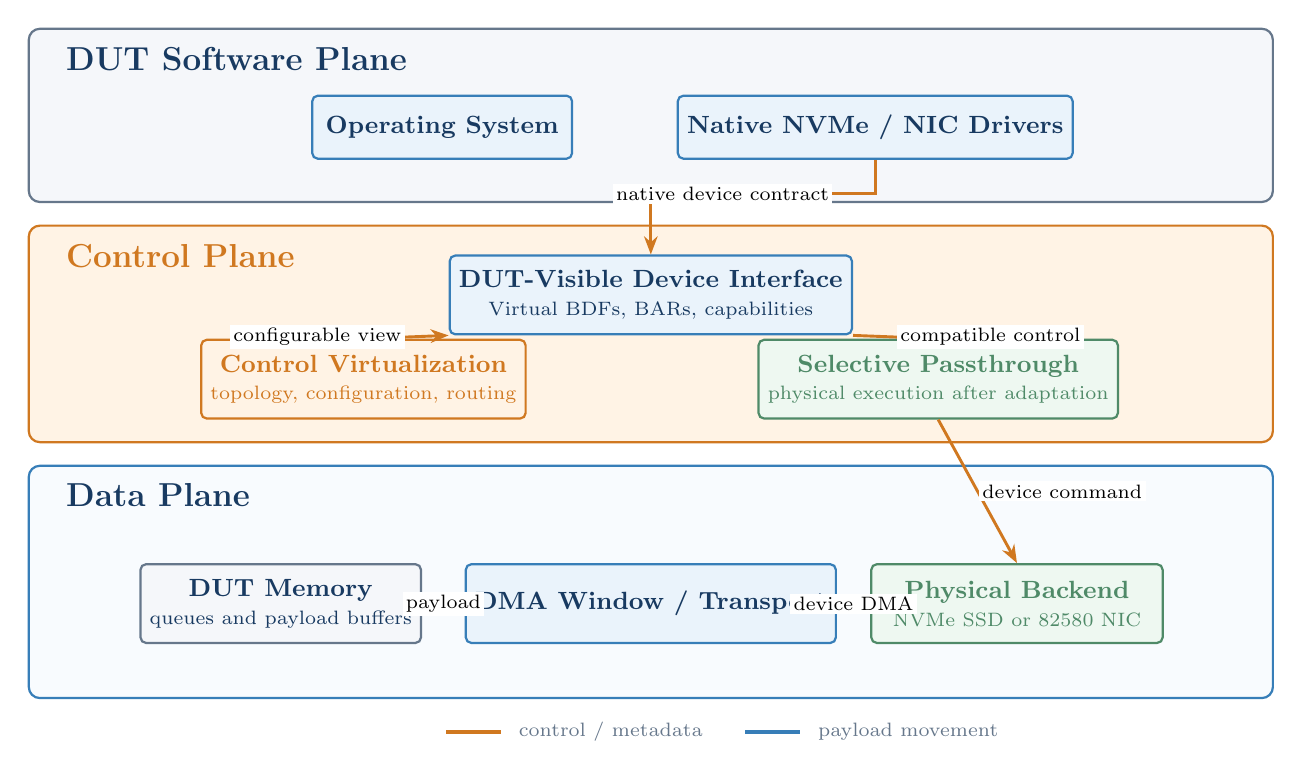
\begin{tikzpicture}[x=1cm,y=1cm]
  \fill[grayfill, rounded corners=4pt] (0,6.3) rectangle (15.8,8.5);
  \draw[slate, line width=.8pt, rounded corners=4pt] (0,6.3) rectangle (15.8,8.5);
  \node[anchor=west, font=\large\bfseries, text=navy] at (.35,8.12) {DUT Software Plane};
  \node[box, minimum width=3.3cm] (os) at (5.25,7.25) {Operating System};
  \node[box, minimum width=3.8cm] (drv) at (10.75,7.25) {Native NVMe / NIC Drivers};

  \fill[orangefill, rounded corners=4pt] (0,3.25) rectangle (15.8,6.0);
  \draw[orange, line width=.8pt, rounded corners=4pt] (0,3.25) rectangle (15.8,6.0);
  \node[anchor=west, font=\large\bfseries, text=orange] at (.35,5.62) {Control Plane};
  \node[box, minimum width=4.5cm, minimum height=10mm] (vif) at (7.9,5.12)
    {DUT-Visible Device Interface\\[-1pt]\normalfont\scriptsize Virtual BDFs, BARs, capabilities};
  \node[controlbox, minimum width=4.0cm, minimum height=10mm] (virt) at (4.25,4.05)
    {Control Virtualization\\[-1pt]\normalfont\scriptsize topology, configuration, routing};
  \node[passbox, minimum width=4.0cm, minimum height=10mm] (pass) at (11.55,4.05)
    {Selective Passthrough\\[-1pt]\normalfont\scriptsize physical execution after adaptation};

  \fill[bluefill!35, rounded corners=4pt] (0,0) rectangle (15.8,2.95);
  \draw[blue, line width=.8pt, rounded corners=4pt] (0,0) rectangle (15.8,2.95);
  \node[anchor=west, font=\large\bfseries, text=navy] at (.35,2.58) {Data Plane};
  \node[mem, minimum width=3.3cm, minimum height=10mm] (memory) at (3.2,1.2)
    {DUT Memory\\[-1pt]\normalfont\scriptsize queues and payload buffers};
  \node[box, minimum width=3.3cm, minimum height=10mm] (dma) at (7.9,1.2)
    {DMA Window / Transport};
  \node[passbox, minimum width=3.7cm, minimum height=10mm] (device) at (12.55,1.2)
    {Physical Backend\\[-1pt]\normalfont\scriptsize NVMe SSD or 82580 NIC};

  \draw[ctrl] (drv.south) -- ++(0,-.43) -| node[elabel, pos=.34] {native device contract} (vif.north);
  \draw[ctrl] (virt.north) -- node[elabel, left] {configurable view} (vif.south west);
  \draw[ctrl] (vif.south east) -- node[elabel, right] {compatible control} (pass.north);
  \draw[ctrl] (pass.south) -- node[elabel, right] {device command} (device.north);
  \draw[data] (memory.east) -- node[elabel] {payload} (dma.west);
  \draw[data] (dma.east) -- node[elabel] {device DMA} (device.west);

  \draw[orange, line width=1.15pt] (5.3,-.43) -- (6.0,-.43);
  \node[anchor=west, font=\scriptsize, text=slate] at (6.1,-.43) {control / metadata};
  \draw[blue, line width=1.4pt] (9.1,-.43) -- (9.8,-.43);
  \node[anchor=west, font=\scriptsize, text=slate] at (9.9,-.43) {payload movement};
\end{tikzpicture}
\end{document}
